% problemas: fundamentos de probabilidad

\section*{Problemas}

La baraja está dividida en cuatro palos (en inglés: suit), dos de color rojo y dos de color negro:
\begin{itemize}
	\item Espadas (conocidas como picas) $\spadesuit$,
	\item Corazones $\heartsuit$,
	\item Rombos (conocidos como diamantes, oros o cocos) $ \diamondsuit$,
	\item Tréboles (conocidos como flores) $\clubsuit$
\end{itemize}

Cada palo está formado por 13 cartas, de las cuales 9 cartas son numerales y 4 literales. Se ordenan de menor a mayor "rango" de la siguiente forma: A, 2, 3, 4, 5, 6, 7, 8, 9, 10, J, Q y K.

\begin{figure}
	\centering
	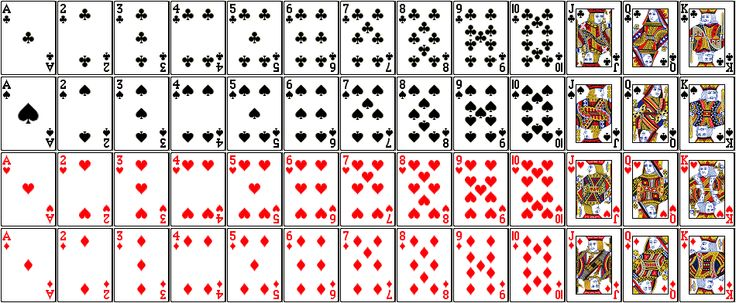
\includegraphics[width=10cm]{./pe/deck.jpg}
	% deck.jpg: 0x0 pixel, 300dpi, 0.00x0.00 cm, bb=
	\caption{Baraja inglesa}
	\label{fig:deck}
\end{figure}



\begin{problema}
	\label{problema:2.1}
	Una carta se obtiene al azar de una baraja inglesa. Describe el espacio muestral si se consideran los palos.
\end{problema}

\begin{solucion}\label{solucion:2.1}
	
	\href{https://youtu.be/4LdLWpQIcBQ}{Consulta también la solución en línea.}
	
	
	La solución está dada por el producto cartesiano del conjunto \[ A = \set{1,2,3,4}, \] donde cada número representa alguno de los palos, y el conjunto \[ B = \set{A,2,...,10,J,Q,K}.\] De manera que el espacio muestral contiene $ 4\times 13=52 $ puntos muestrales. 	
\end{solucion}


\begin{problema}
	\label{problema:2.2}
	Supongamos que $A$ es el evento \texttt{``se obtiene un rey''} o simplemente $\set{K},$ mientras que $B$ es \texttt{``se obtiene un tr\'ebol} o simplemente $\set{\clubsuit}$. Describe los siguiente eventos: 
	\begin{enumerate}
		\item $A\cup B$ 
		\item $A\cap B$ 
		\item $A \cup B'$ 
		\item $A' \cup B'$ 
		\item $A - B$ 
		\item $A'-B'$ 
		\item $(A\cap B) \cup (A\cap B')$
	\end{enumerate}
\end{problema}

\begin{solucion}
	\label{solucion:2.2}
	\href{https://youtu.be/S9VFhMWVyu4}{Consulta también la solución en línea.}
	\begin{enumerate}
		\item Se obtiene un rey o un trébol.
		\item Se obtiene un rey y un trébol.
		\item Se obtiene un rey o no se obtiene un trébol. De manera equivalente: Si se obtiene un trébol, entonces se obtiene un rey. 
		\item No se obtiene un rey o no se obtiene un trébol.
		\item Se obtiene un rey, pero no un trébol. 
		\item No se obtiene un rey ni un trébol.
		\item O bien se obtiene un rey y un trébol, o bien se obtiene un rey pero no un trébol. De manera equivalente: Se obtiene un rey.		
	\end{enumerate}
\end{solucion}



\begin{problema}
	\label{problema:2.3}
	De una baraja inglesa se extraen 2 cartas. Encuentre la probabilidad de que las dos sean ases si la primera carta...
	\begin{enumerate}
		\item ...se devuelve a la baraja.
		\item ...no se devuelve a la baraja.
	\end{enumerate}
	
\end{problema}

\begin{solucion}
	\label{solucion:2.3}
	\begin{enumerate}
		\item \[ \dfrac{4}{52}\times\dfrac{4}{52} = \dfrac{1}{13}\times \dfrac{1}{13} = \dfrac{1}{169} \]
		\item \[ \dfrac{4}{52}\times\dfrac{3}{51} = \dfrac{1}{221} \]
	\end{enumerate}
\end{solucion}


\begin{problema}
	\label{problema:2.4}
	En un contenedor hay 6 pelotas rojas, 4 blancas y 5 azules. Se extraen sucesivamente 3 pelotas. Encuéntrese la probabilidad de que se extraigan en el orden roja, blanca y azul si...
	\begin{enumerate}
		\item ...cada pelota se devuelve a la caja.
		\item ...no se devuelve.
	\end{enumerate}
	
\end{problema}

\begin{solucion}
	\label{solucion:2.4}
	En total, hay 15 pelotas en el contenedor.
	\begin{enumerate}
		\item 
		\[
			\dfrac{6}{15}\times\dfrac{4}{15}\times\dfrac{5}{15}
			=\dfrac{8}{225}.
		\]
	\item
	\[
		\dfrac{6}{15}\times\dfrac{4}{14}\times\dfrac{5}{13}
		=\dfrac{4}{91}.
	\]
	\end{enumerate}
\end{solucion}


\begin{problema}
	\label{problema:2.5}
	Encuéntrese la probabilidad de que en dos lanzamientos de un dado se obtengan por lo menos un 4 en alguno de los dos lanzamientos.
\end{problema}

\begin{solucion}
	\label{solucion:2.5}
	El espacio solución está dado por 
	\[
		E = \set{4,5,6}\times \set{1,..,6} \cup \set{1,...,6}\times\set{4,...,6}
	\]
cuya cardinalidad es $ 9 $. 

Ahora bien, el espacio muestral está dado por
\[
	S = \set{1,...,6}\times\set{1,...,6},
\]
cuya cardinalidad es $ 36 $.

De manera que la probabilidad es 
\[
	\dfrac{9}{36}=\dfrac{1}{4}.
\]

\end{solucion}

\begin{problema}
	\label{problema:2.6}
	Encuentre la probabilidad de no obtener una suma de 7 o de 11 puntos al lanzar ambos dados.
\end{problema}


\begin{solucion}
	\label{solucion:2.6}
	Consideremos nuevamente el espacio muestral 
	\[
		S = \set{1,...,6}\times\set{1,...,6}.
	\]

	Podemos obtener una suma igual con 7 con los siguientes puntos:
	\[
		\set{(1,6),(2,5),(3,4),(4,3),(5,2),(6,1)}, 
	\]
	mientras que la de 11, con los siguientes:
	\[\label{key}
		\set{(5,6), (6,5)}
	\].

	Estos eventos son mutuamente excluyentes (es decir, como conjuntos son disjuntos). Por lo que existen 8 posibles eventos simples con los que obtendríamos o bien una suma de 7 o bien una suma de 11.
	
	Por tanto, la probabilidad es
	\[\label{key}
		1-\dfrac{11}{36}=\dfrac{25}{36}.
	\]
\end{solucion}